\documentclass[../readings.tex]{subfiles}

\begin{document}
\subsection{Principal Component Analysis via SVD}
\label{sub:pca-via-svd}

Principal Component Analysis (PCA) is a fundamental technique for dimensionality reduction. It aims to transform a dataset with many variables into a smaller set of variables, called principal components, while retaining most of the original information or variance. The core idea is to find orthogonal directions in the feature space along which the data exhibits the maximum variance. PCA is widely used for data compression, noise reduction, feature extraction, and visualization. A crucial first step for PCA is data centering.

\addDef{Data Centering}{%
For PCA, the data matrix $\bX \in \mathbb{R}^{n \times p}$ (where $n$ is the number of samples and $p$ is the number of features) must be centered. This means that the mean of each column (feature) is subtracted from all entries in that column, resulting in each feature having a zero mean.
% $$\bX_c = \bX - \mathbf{1}\bar{\bx}^T$$
% where $\mathbf{1}$ is an $n \times 1$ vector of ones and $\bar{\bx}$ is a $p \times 1$ vector of column means.
Throughout this section, $\bX$ will denote a centered data matrix.
}

\addDef{Covariance Matrix}{%
For a centered data matrix $\bX \in \mathbb{R}^{n \times p}$, the sample covariance matrix $\bS$ is defined as:
$$\bS = \frac{1}{n-1} \bX^T \bX$$
where $\bS \in \mathbb{R}^{p \times p}$. The matrix $\bS$ is symmetric and positive semi-definite. Its diagonal entries $S_{jj}$ represent the variance of the $j$-th feature, and its off-diagonal entries $S_{ij}$ represent the covariance between the $i$-th and $j$-th features.
}

\addDef{Principal Component Analysis (PCA)}{%
Given a centered data matrix $\bX \in \mathbb{R}^{n \times p}$, Principal Component Analysis (PCA) seeks to find a new set of orthogonal basis vectors (principal directions) in the $\mathbb{R}^p$ feature space such that the data projected onto these directions has maximal variance. The principal directions are the eigenvectors of the sample covariance matrix $\bS$, ordered according to their corresponding eigenvalues in decreasing order. The eigenvalues represent the variance of the data along these principal directions.
}

\textBox{%
\textbf{Optimization Problem for Principal Directions}
The first principal direction $\bw_1$ is found by solving the following optimization problem:
$$\bw_1 = \arg\max_{\|\bw\|=1} \text{Var}(\bX\bw) = \arg\max_{\|\bw\|=1} \bw^T\bS\bw$$
The solution $\bw_1$ is the eigenvector corresponding to the largest eigenvalue of $\bS$. Subsequent principal directions $\bw_k$ are found by solving:
$$\bw_k = \arg\max_{\|\bw\|=1, \bw \perp \{\bw_1,\ldots,\bw_{k-1}\}} \bw^T\bS\bw$$
This iterative process yields the full eigendecomposition of the covariance matrix $\bS$:
$$\bS = \bV\blambda\bV^T$$
where $\bV = [\bv_1, \bv_2, \ldots, \bv_p]$ is an orthogonal matrix whose columns $\bv_i$ are the eigenvectors of $\bS$ (the principal directions), and $\blambda = \text{diag}(\lambda_1, \lambda_2, \ldots, \lambda_p)$ is a diagonal matrix whose entries are the eigenvalues of $\bS$ (the variances along each principal direction), ordered such that $\lambda_1 \geq \lambda_2 \geq \cdots \geq \lambda_p \geq 0$.
}

\addDef{Principal Component Scores}{%
Once the principal directions $\bV$ are determined, the original centered data $\bX$ can be projected onto these directions to obtain the principal component scores, denoted by $\bZ$:
$$\bZ = \bX\bV$$
The matrix $\bZ \in \mathbb{R}^{n \times p}$ contains the new coordinates of the $n$ data points in the basis defined by the principal directions. The $k$-th column of $\bZ$, denoted $\bz_k = \bX\bv_k$, is called the $k$-th principal component (PC). The sample variance of the $k$-th principal component is $\lambda_k$. The principal components are uncorrelated: $\text{Cov}(\bz_j, \bz_k) = 0$ for $j \neq k$.
}

\addDef{The SVD-PCA Connection}{%
For a centered data matrix $\bX \in \mathbb{R}^{n \times p}$, let its Singular Value Decomposition (SVD) be $\bX = \bU\bsigma\bV^T$. The connection to PCA is as follows:
\begin{itemize}
    \item \textbf{Principal Directions:} The columns of $\bV$ (the right singular vectors of $\bX$) are precisely the principal directions $\bv_i$ (eigenvectors of $\bS$).
    \item \textbf{Variances:} The squared singular values of $\bX$, denoted $\sigma_i^2$, are related to the eigenvalues $\lambda_i$ of $\bS$ by $\lambda_i = \frac{\sigma_i^2}{n-1}$. Thus, $\sigma_i^2/(n-1)$ is the variance explained by the $i$-th principal component.
    \item \textbf{Principal Component Scores:} The principal component scores $\bZ = \bX\bV$ can be directly computed using the SVD as $\bZ = \bU\bsigma$. (Assuming $\bU$ is $n \times p$ and $\bsigma$ is $p \times p$ for $n \ge p$, or more generally, $\bU$ is $n \times r$, $\bsigma$ is $r \times r$, $\bV$ is $p \times r$ where $r = \text{rank}(\bX)$).
\end{itemize}
This connection highlights that PCA can be performed directly using the SVD of $\bX$, often providing better numerical stability than forming and diagonalizing $\bS$.
}

\textBox{Derivation of the SVD-PCA Connection}{%
To establish this connection, substitute the SVD of $\bX$ into the formula for the covariance matrix $\bS$:
\begin{align}
\bS &= \frac{1}{n-1}\bX^T\bX \nonumber \\
&= \frac{1}{n-1}(\bU\bsigma\bV^T)^T(\bU\bsigma\bV^T) \nonumber \\
&= \frac{1}{n-1}(\bV\bsigma^T\bU^T)(\bU\bsigma\bV^T) \nonumber \\
&= \frac{1}{n-1}\bV\bsigma^T(\bU^T\bU)\bsigma\bV^T
\end{align}
Assuming the "economy" SVD where $\bU$ has orthonormal columns (i.e., $\bU^T\bU = \bI_r$, where $r = \text{rank}(\bX)$ is the number of non-zero singular values, typically $r=p$ if $n \ge p$ and $\bX$ has full column rank), and $\bsigma$ is an $r \times r$ diagonal matrix of singular values $\sigma_i$, then $\bsigma^T\bsigma = \bsigma^2$. The equation becomes:
$$ \bS = \frac{1}{n-1}\bV\bsigma^2\bV^T $$
Comparing this with the eigendecomposition of $\bS = \bV\blambda\bV^T$, we see that the columns of $\bV$ are the eigenvectors of $\bS$, and the eigenvalues $\lambda_i$ are given by $\lambda_i = \frac{\sigma_i^2}{n-1}$.
}

\addDef{Dimensionality Reduction via PCA}{%
PCA is often used to reduce the dimensionality from $p$ features to $k < p$ principal components. The first $k$ principal components $\bZ_k = \bX\bV_k = \bU_k\bsigma_k$ (where $\bV_k$ contains the first $k$ columns of $\bV$, $\bU_k$ the first $k$ columns of $\bU$, and $\bsigma_k$ the top-left $k \times k$ block of $\bsigma$) capture the most variance.
The rank-$k$ approximation of the original data $\bX$ using the first $k$ principal components is:
$$\bX_k = \bZ_k\bV_k^T = \bX\bV_k\bV_k^T = \bU_k\bsigma_k\bV_k^T$$
This matrix $\bX_k$ represents the projection of the original data onto the subspace spanned by the first $k$ principal directions. By the Eckart-Young-Mirsky theorem, $\bX_k$ is the best rank-$k$ approximation of $\bX$ in terms of Frobenius norm, meaning it minimizes $\|\bX-\bA\|_F^2$ among all rank-$k$ matrices $\bA$.
}

\addExmpl{%
Consider a centered data matrix $\bX \in \mathbb{R}^{100 \times 3}$ representing 100 3D points ($n=100, p=3$). Suppose the singular values of $\bX$ are $\sigma_1 = 10\sqrt{n-1}$, $\sigma_2 = 5\sqrt{n-1}$, $\sigma_3 = 0.5\sqrt{n-1}$. The corresponding eigenvalues of $\bS$ would be $\lambda_1 = \sigma_1^2/(n-1) = 100$, $\lambda_2 = 25$, $\lambda_3 = 0.25$.

\begin{itemize}
    \item The proportion of total variance explained by the first principal component is:
    $$ \frac{\lambda_1}{\lambda_1 + \lambda_2 + \lambda_3} = \frac{100}{100 + 25 + 0.25} = \frac{100}{125.25} \approx 0.798 $$
    \item The condition number of the covariance matrix $\bS$ (assuming $\lambda_3 > 0$) is:
    $$ \kappa(\bS) = \frac{\lambda_{\text{max}}}{\lambda_{\text{min}}} = \frac{\lambda_1}{\lambda_3} = \frac{100}{0.25} = 400 $$
\end{itemize}
A rank-2 approximation $\bX_2$ would use the first two principal components. The proportion of variance captured by these two components is:
$$ \frac{\lambda_1 + \lambda_2}{\lambda_1 + \lambda_2 + \lambda_3} = \frac{100 + 25}{125.25} = \frac{125}{125.25} \approx 0.998 $$
This indicates that the data is nearly coplanar, as approximately 99.8\% of the variance is contained within a 2D subspace.
}

\addDef{Error Analysis and Choosing $k$}{%
The reconstruction error from truncating to $k$ principal components, i.e., using $\bX_k$ to approximate $\bX$, is given by the sum of the neglected singular values squared:
$$\|\bX - \bX_k\|_F^2 = \sum_{i=k+1}^{r} \sigma_i^2$$
where $r = \text{rank}(\bX)$. In terms of eigenvalues of $\bS$, this is $(n-1)\sum_{i=k+1}^{r} \lambda_i$.

The choice of $k$ (the number of principal components to retain) depends on the application. Common methods include:
\begin{itemize}
    \item \textbf{Proportion of Variance Explained (PVE):} Choose $k$ such that the cumulative PVE reaches a desired threshold (e.g., 90\%, 95\%). The PVE for $k$ components is:
    $$ \text{PVE}_k = \frac{\sum_{i=1}^k \lambda_i}{\sum_{i=1}^p \lambda_i} = \frac{\sum_{i=1}^k \sigma_i^2}{\sum_{i=1}^p \sigma_i^2} $$
    (Assuming $\sum \sigma_i^2 \neq 0$).
    \item \textbf{Scree Plot:} Plot the eigenvalues $\lambda_i$ (or singular values $\sigma_i$) in decreasing order. Look for an "elbow" or a point where the values level off. Components beyond this point might represent noise.
    \item \textbf{Application-specific criteria:} The choice of $k$ might also be guided by the needs of a downstream task, such as visualization ($k=2$ or $k=3$) or computational constraints.
\end{itemize}
}


\addNote{%
The SVD $\bX = \bU\bsigma\bV^T$ offers a powerful geometric interpretation of PCA. The columns of $\bV$ (principal directions) form an orthonormal basis for the feature space $\mathbb{R}^p$. The transformation $\bX \to \bX\bV = \bU\bsigma$ projects the data points onto this new basis, yielding the principal component scores. The singular values $\sigma_i$ (related to $\sqrt{\lambda_i}$) indicate the "stretch" or importance of each principal direction in terms of data variance. $\bU$ contains an orthonormal basis for the column space of $\bX$, representing the principal component scores in a rotated coordinate system in $\mathbb{R}^n$.
}

\addParagraph{
For a visualization of principal directions, the figure below (conceptual) illustrates how the right singular vectors from SVD (columns of $\bV$) correspond to the principal directions of a 2D dataset. These vectors are typically scaled by their corresponding singular values (or square root of eigenvalues) to indicate the magnitude of variance along each direction.

% Suggestion for TikZ visualization of principal directions
 \begin{center}
 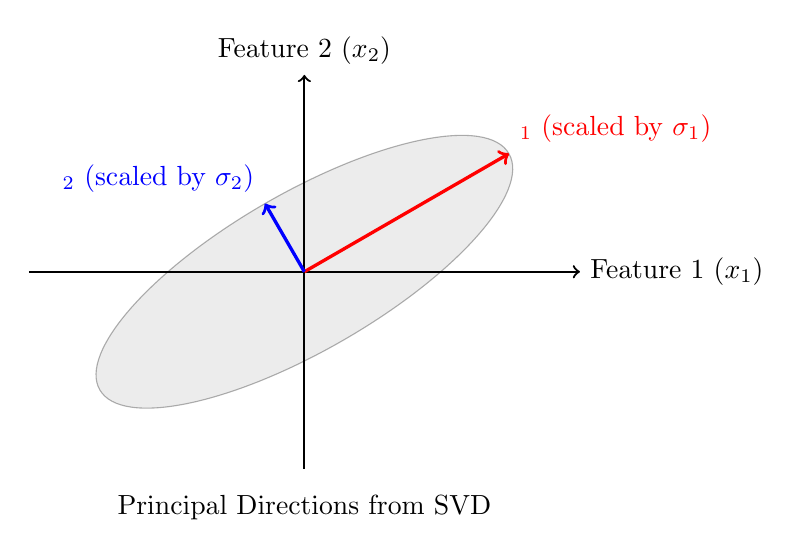
\begin{tikzpicture}
   % Draw data points as a cloud (example)
   \path[fill=lightgray, opacity=0.3, draw=black, thin, rotate=30] (0,0) ellipse (3cm and 1cm);
   % Draw coordinate axes
   \draw[->,thick] (-3.5,0) -- (3.5,0) node[right] {Feature 1 ($x_1$)};
   \draw[->,thick] (0,-2.5) -- (0,2.5) node[above] {Feature 2 ($x_2$)};
   % Draw principal components as vectors (example directions and lengths)
   % Assume \sigma_1 > \sigma_2
   \draw[->,very thick,red] (0,0) -- ({3*cos(30)},{3*sin(30)}) node[anchor=south west] {$\bv_1$ (scaled by $\sigma_1$)}; % PC1
   \draw[->,very thick,blue] (0,0) -- ({-1*sin(30)},{1*cos(30)}) node[anchor=south east] {$\bv_2$ (scaled by $\sigma_2$)}; % PC2
   \node at (0,-3) {Principal Directions from SVD};
 \end{tikzpicture}
\end{center}
PCA effectively rotates the original coordinate system to a new one aligned with the directions of maximum variance.
}


\addDef{Relationship to Eigendecomposition}{%
The SVD of $\bX$ is intrinsically linked to the eigendecompositions of $\bX^T\bX$ and $\bX\bX^T$:
\begin{align}
(\bX^T\bX)\bV &= \bV\bsigma^T\bsigma = \bV\bsigma_p^2 \nonumber \\
(\bX\bX^T)\bU &= \bU\bsigma\bsigma^T = \bU\bsigma_n^2
\end{align}
where $\bsigma_p^2$ is a $p \times p$ diagonal matrix with diagonal entries $\sigma_i^2$ (and zeros if $p > r$), and $\bsigma_n^2$ is an $n \times n$ diagonal matrix with diagonal entries $\sigma_i^2$ (and zeros if $n > r$).
This shows that the right singular vectors $\bv_i$ (columns of $\bV$) are eigenvectors of $\bX^T\bX$, and the left singular vectors $\bu_i$ (columns of $\bU$) are eigenvectors of $\bX\bX^T$. The eigenvalues of both $\bX^T\bX$ and $\bX\bX^T$ are $\sigma_i^2$.

\textbf{Computational Aspect for High Dimensions ($p \gg n$):}
When the number of features $p$ is much larger than the number of samples $n$, computing $\bS$ (a $p \times p$ matrix) and its eigenvectors can be prohibitively expensive. Instead, one can compute the eigenvectors of the smaller $n \times n$ matrix $\bK_G = \bX\bX^T$ (sometimes called the Gram matrix).
If $\bu_i$ is an eigenvector of $\bX\bX^T$ with eigenvalue $\sigma_i^2$:
$$ \bX\bX^T\bu_i = \sigma_i^2\bu_i $$
Pre-multiplying by $\bX^T$:
$$ \bX^T(\bX\bX^T\bu_i) = \bX^T(\sigma_i^2\bu_i) \implies (\bX^T\bX)(\bX^T\bu_i) = \sigma_i^2(\bX^T\bu_i) $$
This shows that if $\bu_i$ is an eigenvector of $\bX\bX^T$, then $\bX^T\bu_i$ is an eigenvector of $\bX^T\bX$ (i.e., a principal direction).
Thus, for $\sigma_i \neq 0$, we can obtain the principal directions $\bv_i$ by:
$$ \bv_i = \frac{1}{\sigma_i} \bX^T\bu_i $$
The principal component scores can then be found as $\bZ = \bU\bsigma$. The columns of $\bU$ are the eigenvectors of $\bX\bX^T$, and $\bsigma$ contains the square roots of its eigenvalues.
}




\addDef{Statistical Properties of PCA}{%
\begin{itemize}
    \item \textbf{Loadings:} The entries of the principal directions $\bv_j$ (eigenvectors of $\bS$) are called loadings. The loading $v_{ji}$ (the $j$-th element of $\bv_i$) quantifies the contribution of the $j$-th original feature to the $i$-th principal component. A large absolute value of $v_{ji}$ indicates that the $j$-th feature is important for the $i$-th principal component.
    \item \textbf{Correlation with Principal Components:} If the original data $\bX$ is standardized (each feature has zero mean and unit variance), then the loading $v_{ji}$ is the correlation coefficient between the $j$-th original feature and the $i$-th principal component score $\bz_i$.
    \item \textbf{Proportion of Variance Explained (PVE):} As mentioned earlier, PVE by the first $k$ principal components is $\frac{\sum_{i=1}^k \lambda_i}{\sum_{i=1}^p \lambda_i} = \frac{\sum_{i=1}^k \sigma_i^2}{\sum_{i=1}^p \sigma_i^2}$. This is a key metric for assessing how much information is retained after dimensionality reduction.
\end{itemize}
}

\addNote{%
PCA is sensitive to the relative scaling of the original features. Features with larger variances will tend to dominate the first few principal components, even if their variance is due to units of measurement rather than inherent importance. Therefore, it is standard practice to standardize the data before applying PCA, i.e., scale each feature to have unit variance (in addition to zero mean). However, if features are measured in the same units and their relative variances are meaningful, one might choose not to scale.
}

\addNote{%
\begin{itemize}
    \item \textbf{Linearity:} PCA assumes that the principal components are linear combinations of the original features and that the underlying subspace is linear. It may not capture non-linear structures effectively (Kernel PCA can address this).
    \item \textbf{Variance as Importance:} PCA assumes that directions with high variance are the most important. This may not always be true, especially in supervised learning contexts where directions that best separate classes might have small variance.
    \item \textbf{Orthogonality:} The principal components are orthogonal by construction. While this ensures they are uncorrelated and provides a unique basis, real-world underlying factors may not be orthogonal.
    \item \textbf{Interpretation:} While loadings help, interpreting principal components can sometimes be challenging as they are combinations of all original features.
    \item \textbf{Sensitivity to Outliers:} PCA is sensitive to outliers in the data, as they can disproportionately influence the mean and variance calculations.
\end{itemize}
The effectiveness of PCA often hinges on whether the data's intrinsic dimensionality is lower than $p$ and whether directions of high variance are indeed the most informative for the problem at hand. The rapid decay of singular values (or eigenvalues) often indicates that PCA will be effective for dimensionality reduction.
}



\end{document}